\documentclass[10pt]{article}
%\usepackage{epsf}
\usepackage{epsfig}

%\usepackage{alg,alg2}
%\input{psfig.sty}

\usepackage[usenames]{color}
%\input{preamble-isca}
\setcounter{secnumdepth}{4}

\textheight 9in         % 1in top and bottom margin
\textwidth 6.5in        % 1in left and right margin

\oddsidemargin 0in      % Both side margins are now 1in
\evensidemargin 0in \topmargin -0.5 in

% The header goes .5in from top of the page and from the text.

\begin{document}

\normalsize
\bibliographystyle{alpha}


\clearpage
\pagenumbering{arabic}

\title{Investigating Network Testbed Usage}
\author{Jelena Mirkovic, Hao Shi, Alefiya Hussain and Ted Faber\\
USC/ISI\\
\{sunshine, haoshi, hussain, faber\}@isi.edu
}

\maketitle
\begin{abstract}
\end{abstract}
\section{Introduction}

These are key questions that we're seeking to answer:
\begin{enumerate} 
\item Do testbeds help people conduct useful research?
\item What aspects of testbeds hinder their wider use?
\item Can testbed use/management policies be improved and how?
\end{enumerate}
Most of the findings reported here relate to questions 1 and 3. Unfortunately testbeds today
do not collect enough data nor do they collect the right data to answer the above questions
conclusively so we are often forced to draw bold conclusions based on our interpretation of the
existing, limited data.

We observe that there are three primary types of experimentation patterns 
 on testbeds today: (a) {\bf Hypothesis Validation} where the experimenter
 rigorously explores the parameter space to validate 
  a particular hypothesis. 
(b) {\bf Deployment Study} where the experimenter 
 installs new technology to study its impact and/or to test it out
(c) {\bf Exploration} where the experimenter takes 
 unknown technology and immerses it into the testbed to study it further.

In the subsequent sections, we have classified 
 all three cases of experimentation patterns as 
{\it research} experiments. 
Additionally, we have {\it class} experiments
 on DETER, that are instantiated due to use of DETER in graduate and undergraduate
 security courses across 22 universities world-wide. Testbed is also used for internal
 testing -- we exclude all data of such experiments and users from our statistics.


\section{Related Work}

\section{Network Testbeds}

\section{User Diversity}

Testbed use evolves after a few years to outsider-dominant

Class use grows easily

Most users are in US, as expected

\section{Testbed Usage Patterns}

\textbf{Hypothesis:} People use testbeds in multiple visits. Some experiments are small because they are exploring the space

\subsection{Experiment and Project measures}

{\color{red} clustering TODO}


\subsubsection{Experiment Duration}
 {\it Experiment duration} is defined 
 as the time lapse between
  when an experiment is allocated 
   testbed resources 
 to when the experiment releases
  the assigned resources.
Figure~\ref{exdur} shows the \textit{cummulative distribution function (cdf)} of
 duration for our two 
  experiment categories, research and class
   experiments. 
Since each allocation is plotted as an 
 independent event, the same experiment (identified by its name) can generate multiple
 points in Figure~\ref{exdur} if it allocated and released resources multiple times in the course
 of its lifetime.
Research experiment duration is heavy-tailed with 26\% of experiments
lasting less than 15 minutes, 51\% lasting less than 1.5 h and 90\%
lasting less than a day. But a few experiments last more than a year. 
Class experiment duration is also heavy tailed but longer experiments
dominate more: only less than 7\% last less than 15 minutes, 35\% last
less than 1.5 h and 96\% last less than a day. Longest class experiments
last for a few weeks. We attribute this longer duration of class
experiments when compared with research experiments to the fact that
class experiments are usually well specified in advance by the class
instructor. Class users can thus just allocate resources for the experiment and do
useful work, while research users may need several trial resource
allocations while they test out their set up and discover the combination
that best works for their research purpose.

\begin{figure}[htbp]
\begin{center}
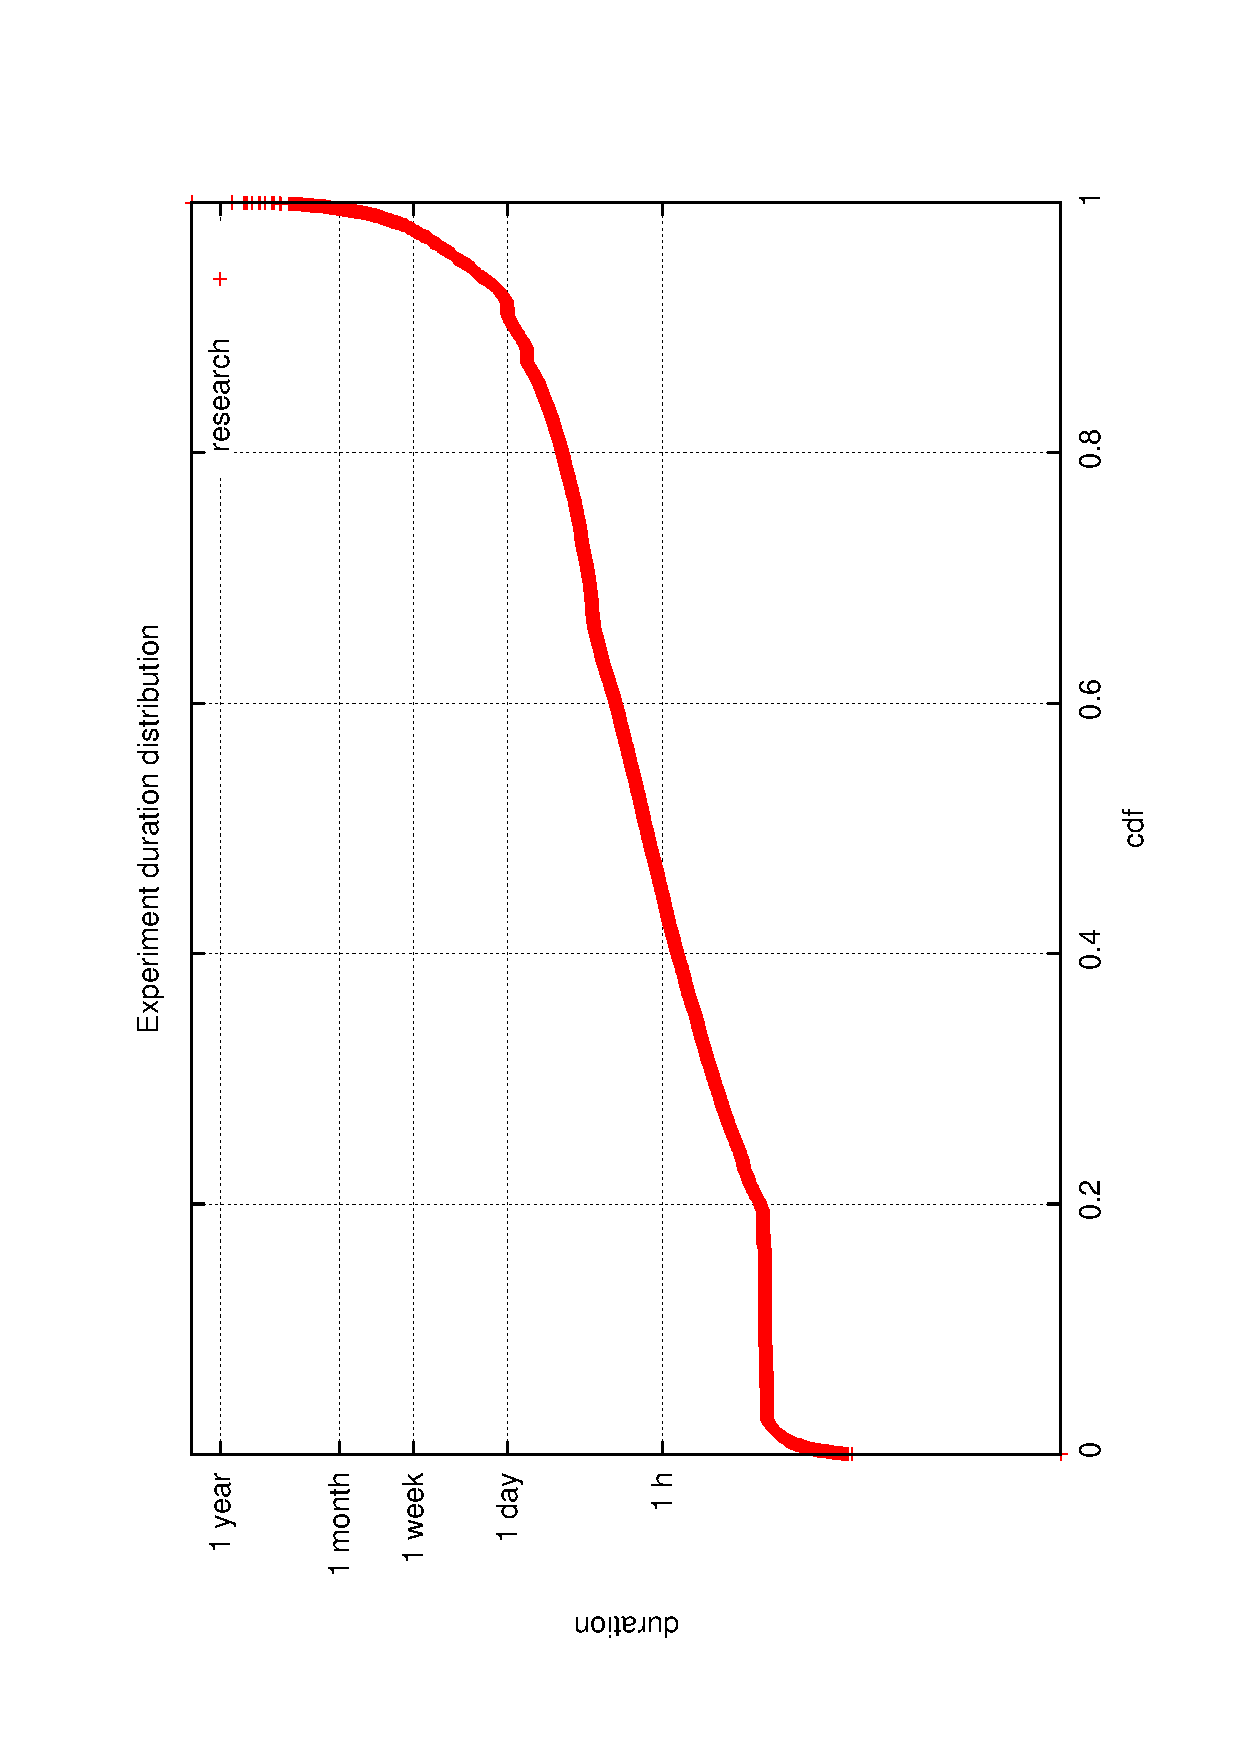
\includegraphics[width=5in]{figs/exdur.pdf}
\caption{Experiment duration distribution}
\label{exdur}
\end{center}
\end{figure}

We also sought to correlate experiment duration and size, which is shown in figures  \ref{dvss} and \ref{cvdss}. As it can be seen, there is no obvious correlation.


\begin{figure}[htbp]
\begin{center}
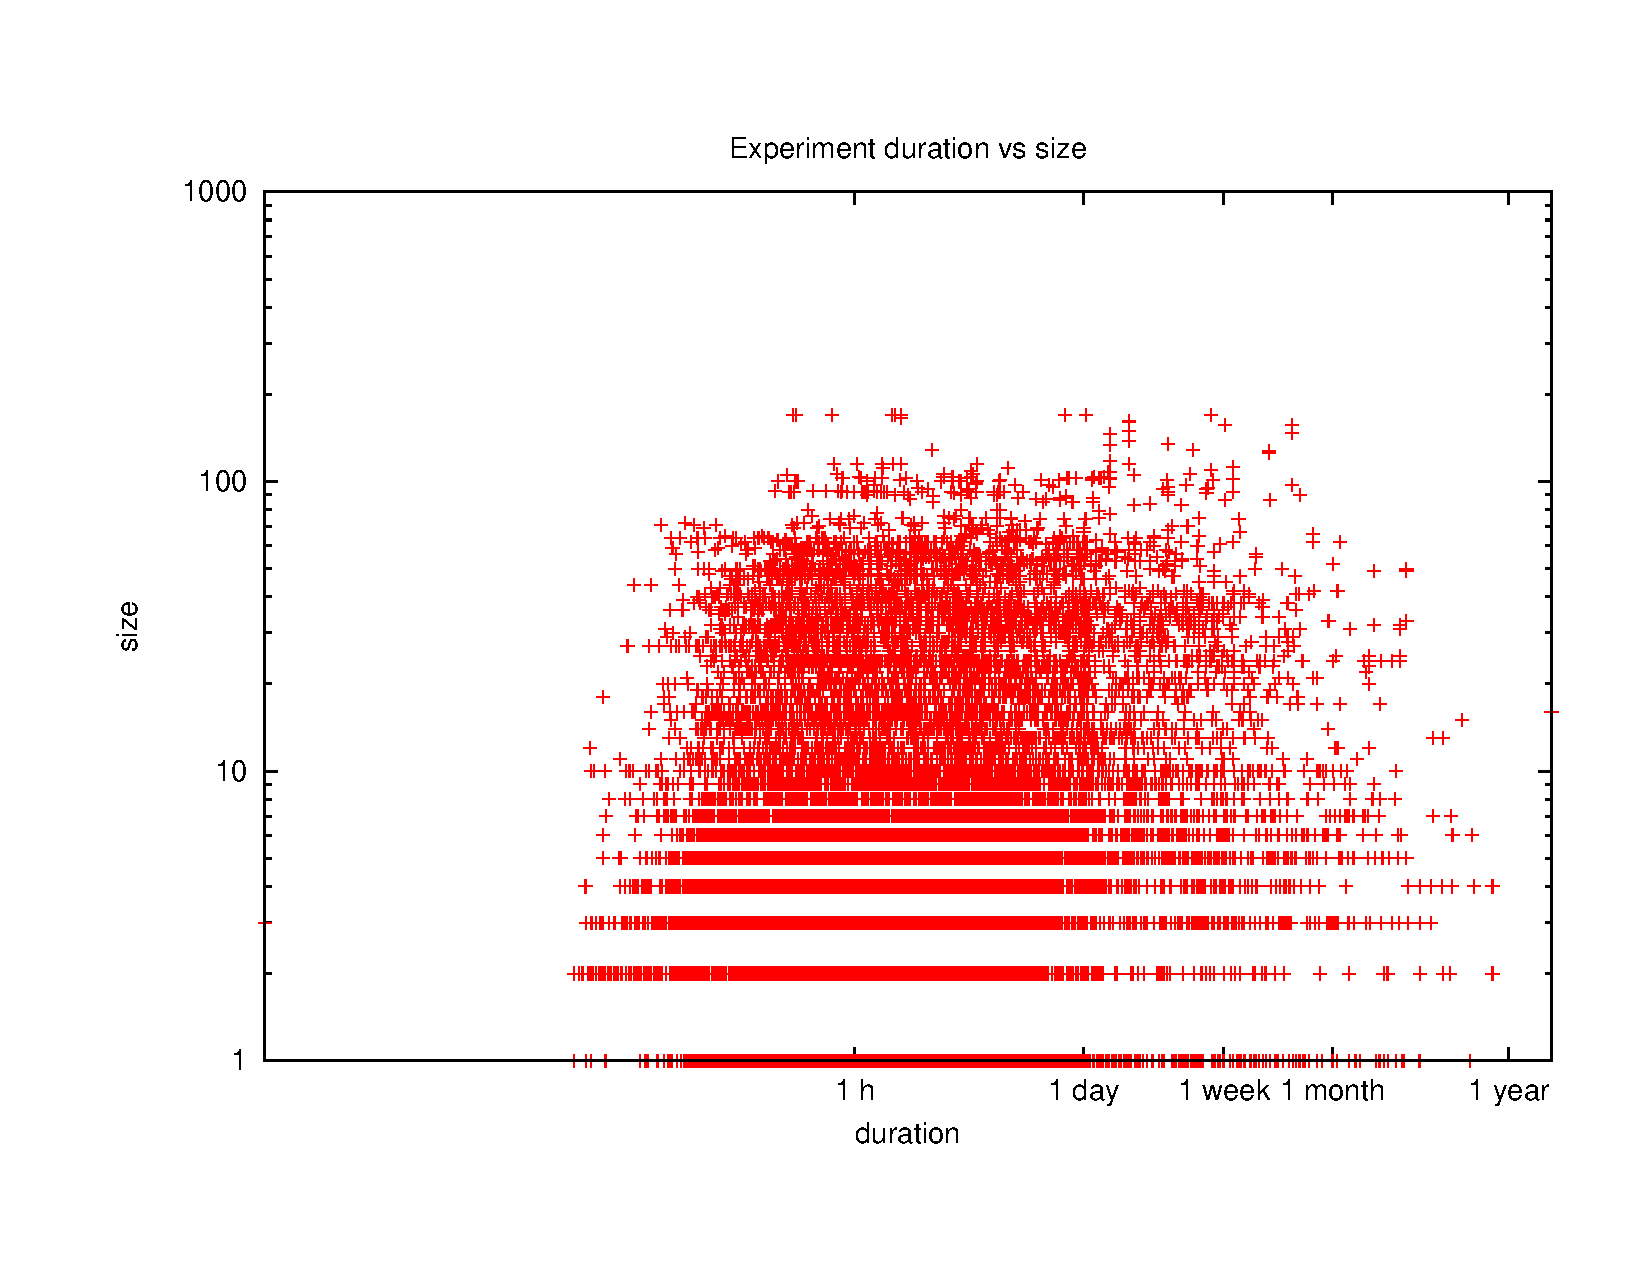
\includegraphics[width=5in]{figs/dvss.pdf}
\caption{Research: Experiment duration vs size}
\label{dvss}
\end{center}
\end{figure}

\begin{figure}[htbp]
\begin{center}
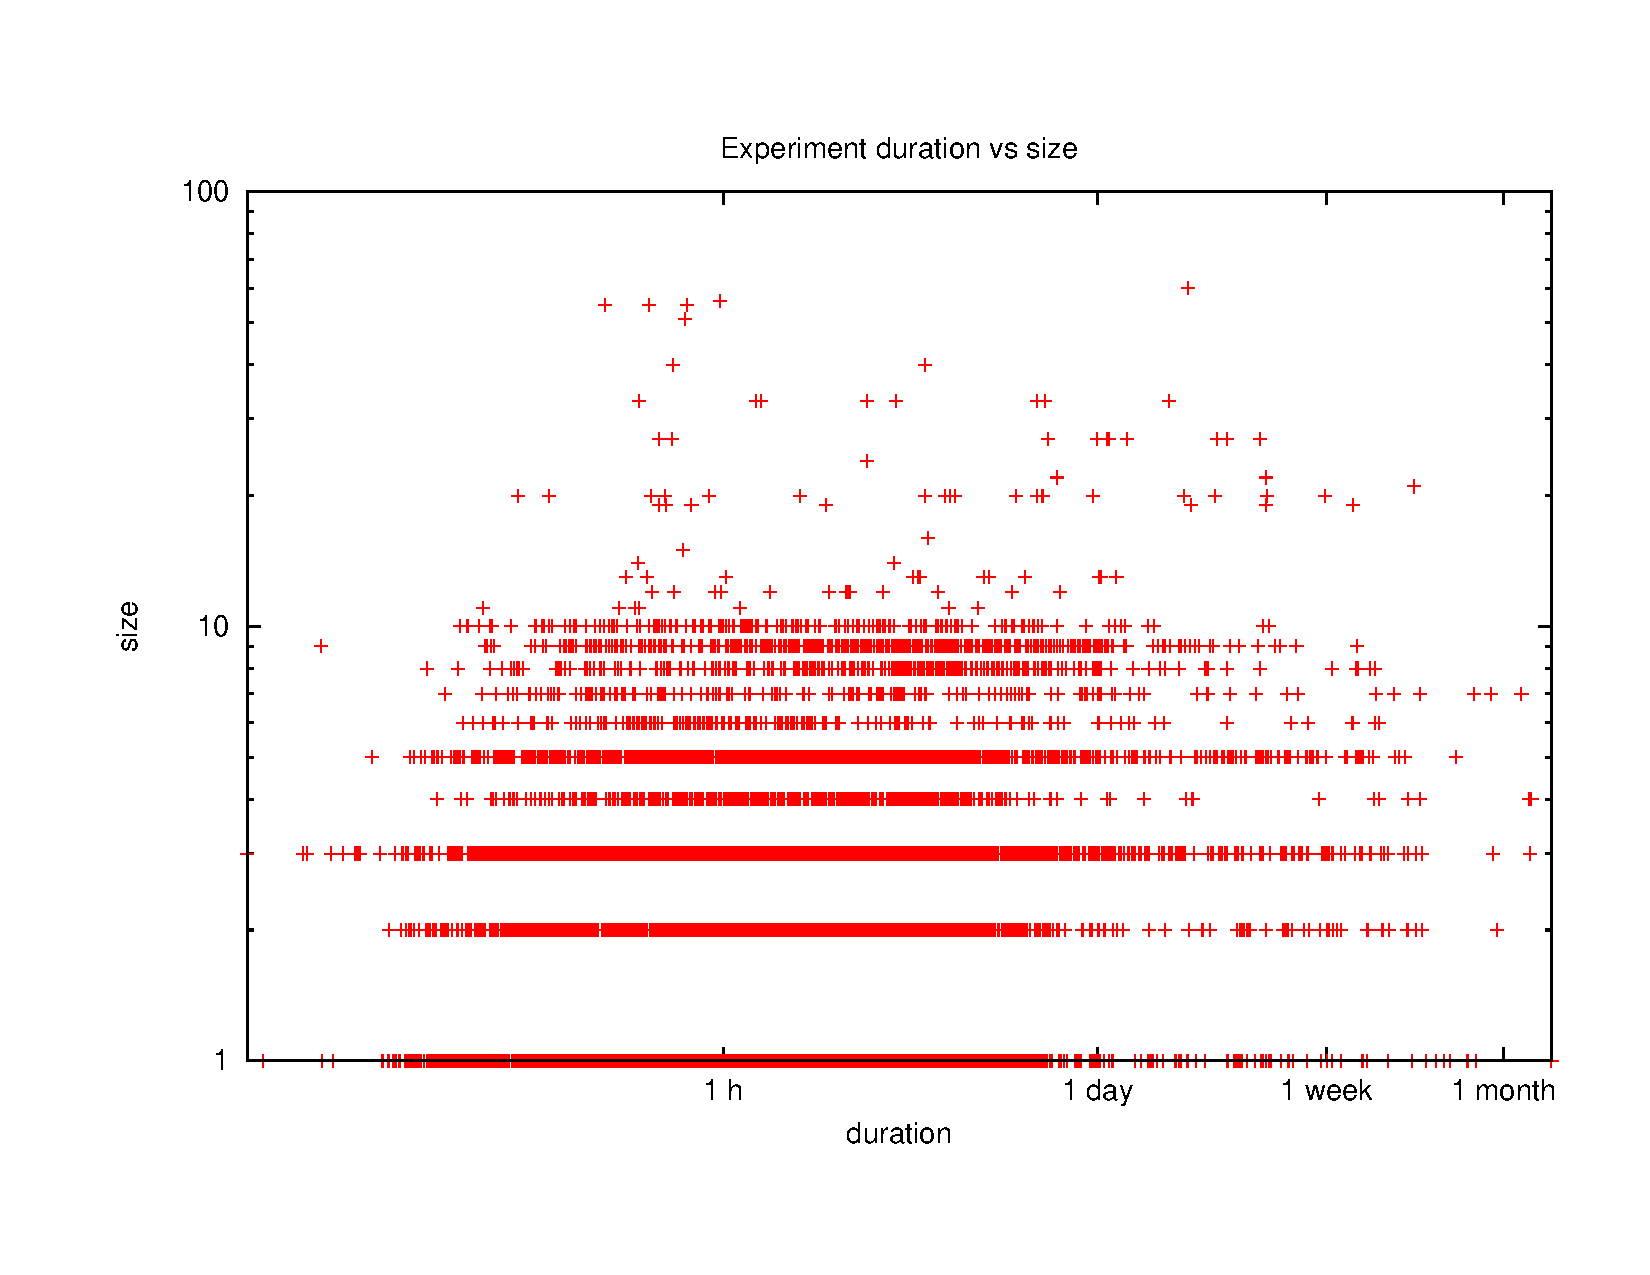
\includegraphics[width=5in]{figs/cdvss.pdf}
\caption{Class: Experiment duration vs size}
\label{cdvss}
\end{center}
\end{figure}


\subsubsection{Experiment Lifetime}
{\it Experiment Lifetime} is defined as 
 time lapse between the first experiment creation
event to the last experiment deallocation event. 
Thus each unique experiment is only represented by one point in 
Figure~\ref{exlife}. 
Research experiment life is heavy-tailed with almost
51\% of experiments lasting less than 10 minutes. Conversely, only 1.4\%
of class experiments last less than 10 minutes. To verify our hypothesis
that short research experiment life is due to users trying to determine
the best setting for their purpose we examined the percentage of short
experiments that are followed by longer experiments in the same project.
If we define "short" as lasting 10 minutes or less 3,835 out of 3,846
(or 99\%) short research experiments are followed by a longer experiment
in the same project. Similarly, we investigated how many short
experiments are preceded by a long experiment, hypothesizing that this
is due to the user perfecting their scripts and automating the
experiment so that it can run under 10 minutes. This time  3,839 out of
3,846 (or 99\%) short research experiments were preceded by a longer
experiment. We conclude that short research experiments occur often in
the middle of experimentation stream when users want to either
investigate new setup or they have sufficiently automated their
experiments that they can finish quickly.


\begin{figure}[htbp]
\begin{center}
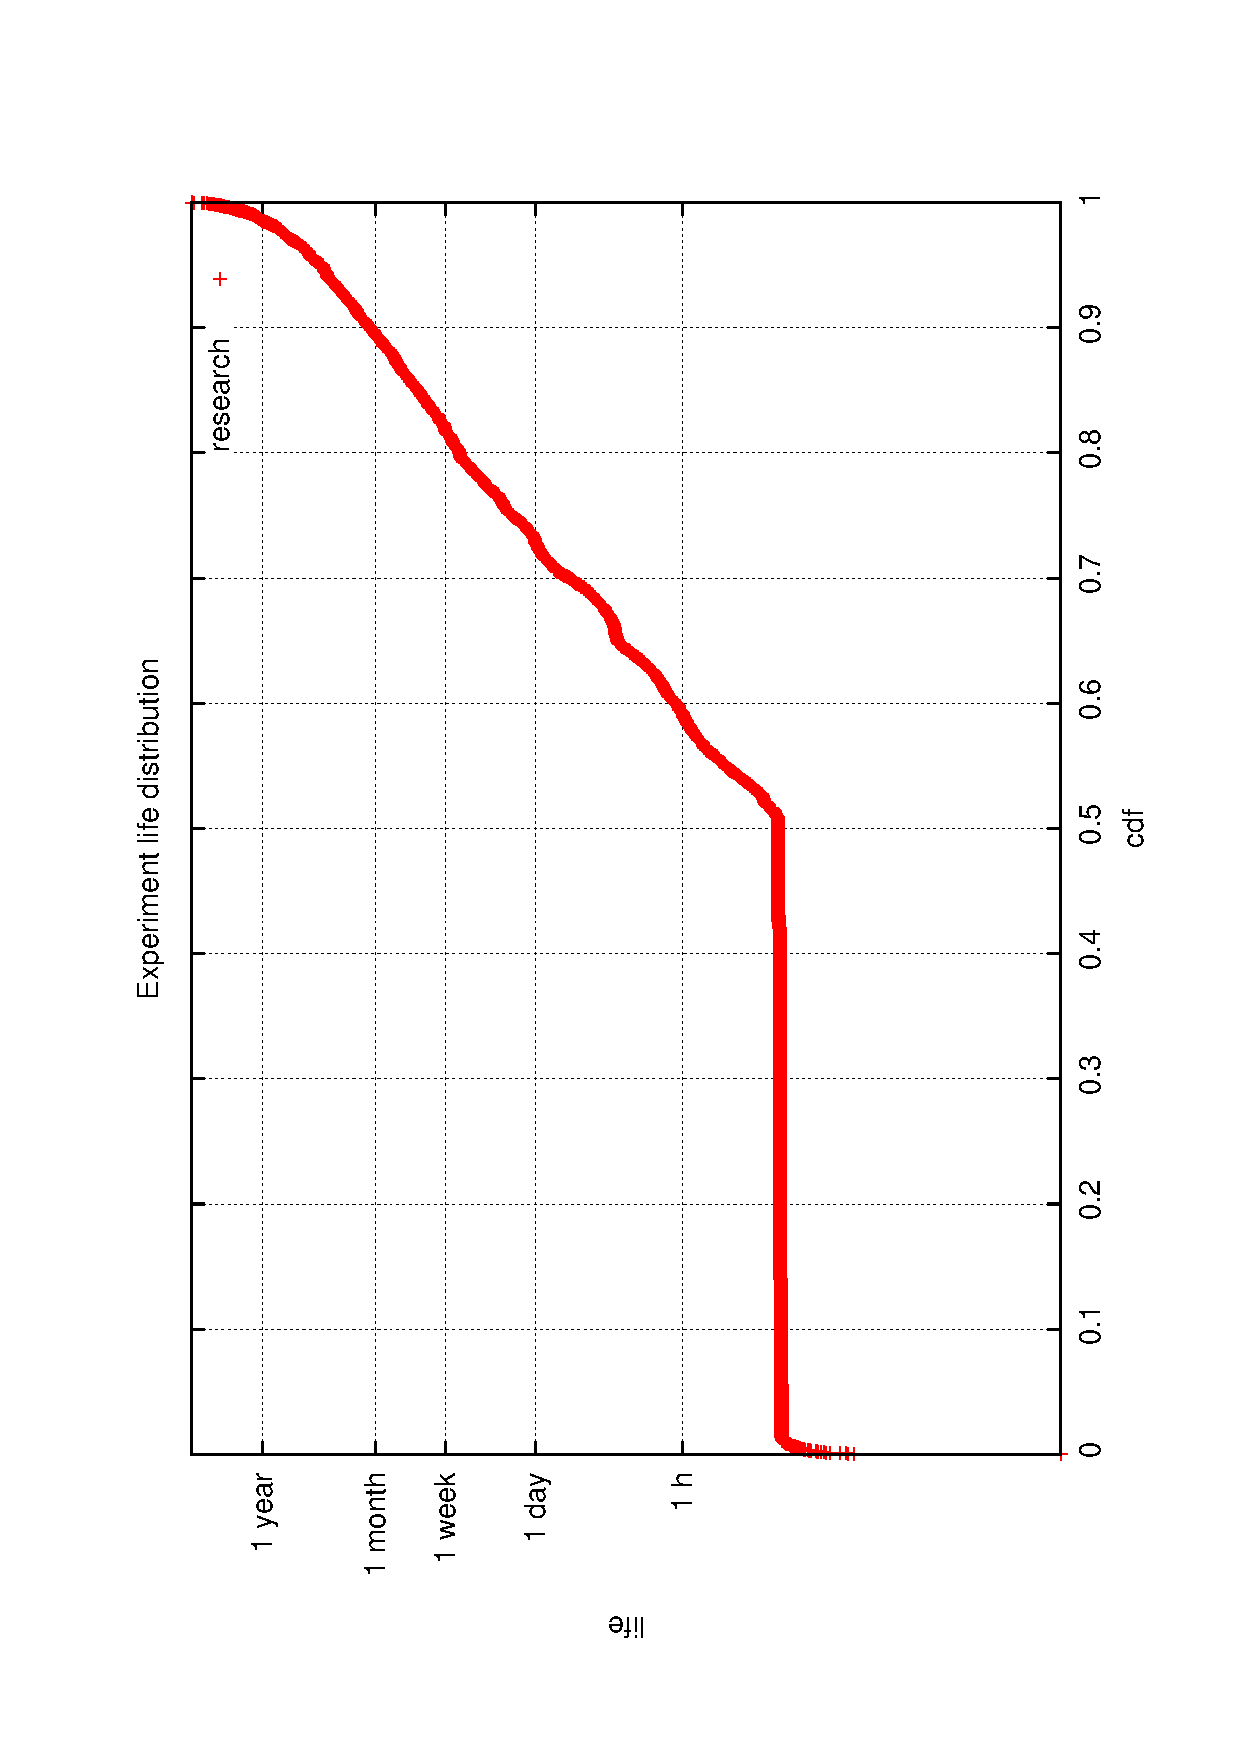
\includegraphics[width=5in]{figs/exlife.pdf}
\caption{Experiment life distribution}
\label{exlife}
\end{center}
\end{figure}

To validate this theory that short experiments are somehow related to longer, more useful
experiments we investigated the minimum elapsed time between a short experiment and 
a longer one either following it or preceding it. Figure \ref{gaps} shows the \textit{cdf} of
these time intervals. About half of the short experiments are performed within an hour of
a longer experiment, and 96\% are performed within a day of a longer experiment. This validates 
our theory.

\begin{figure}[htbp]
\begin{center}
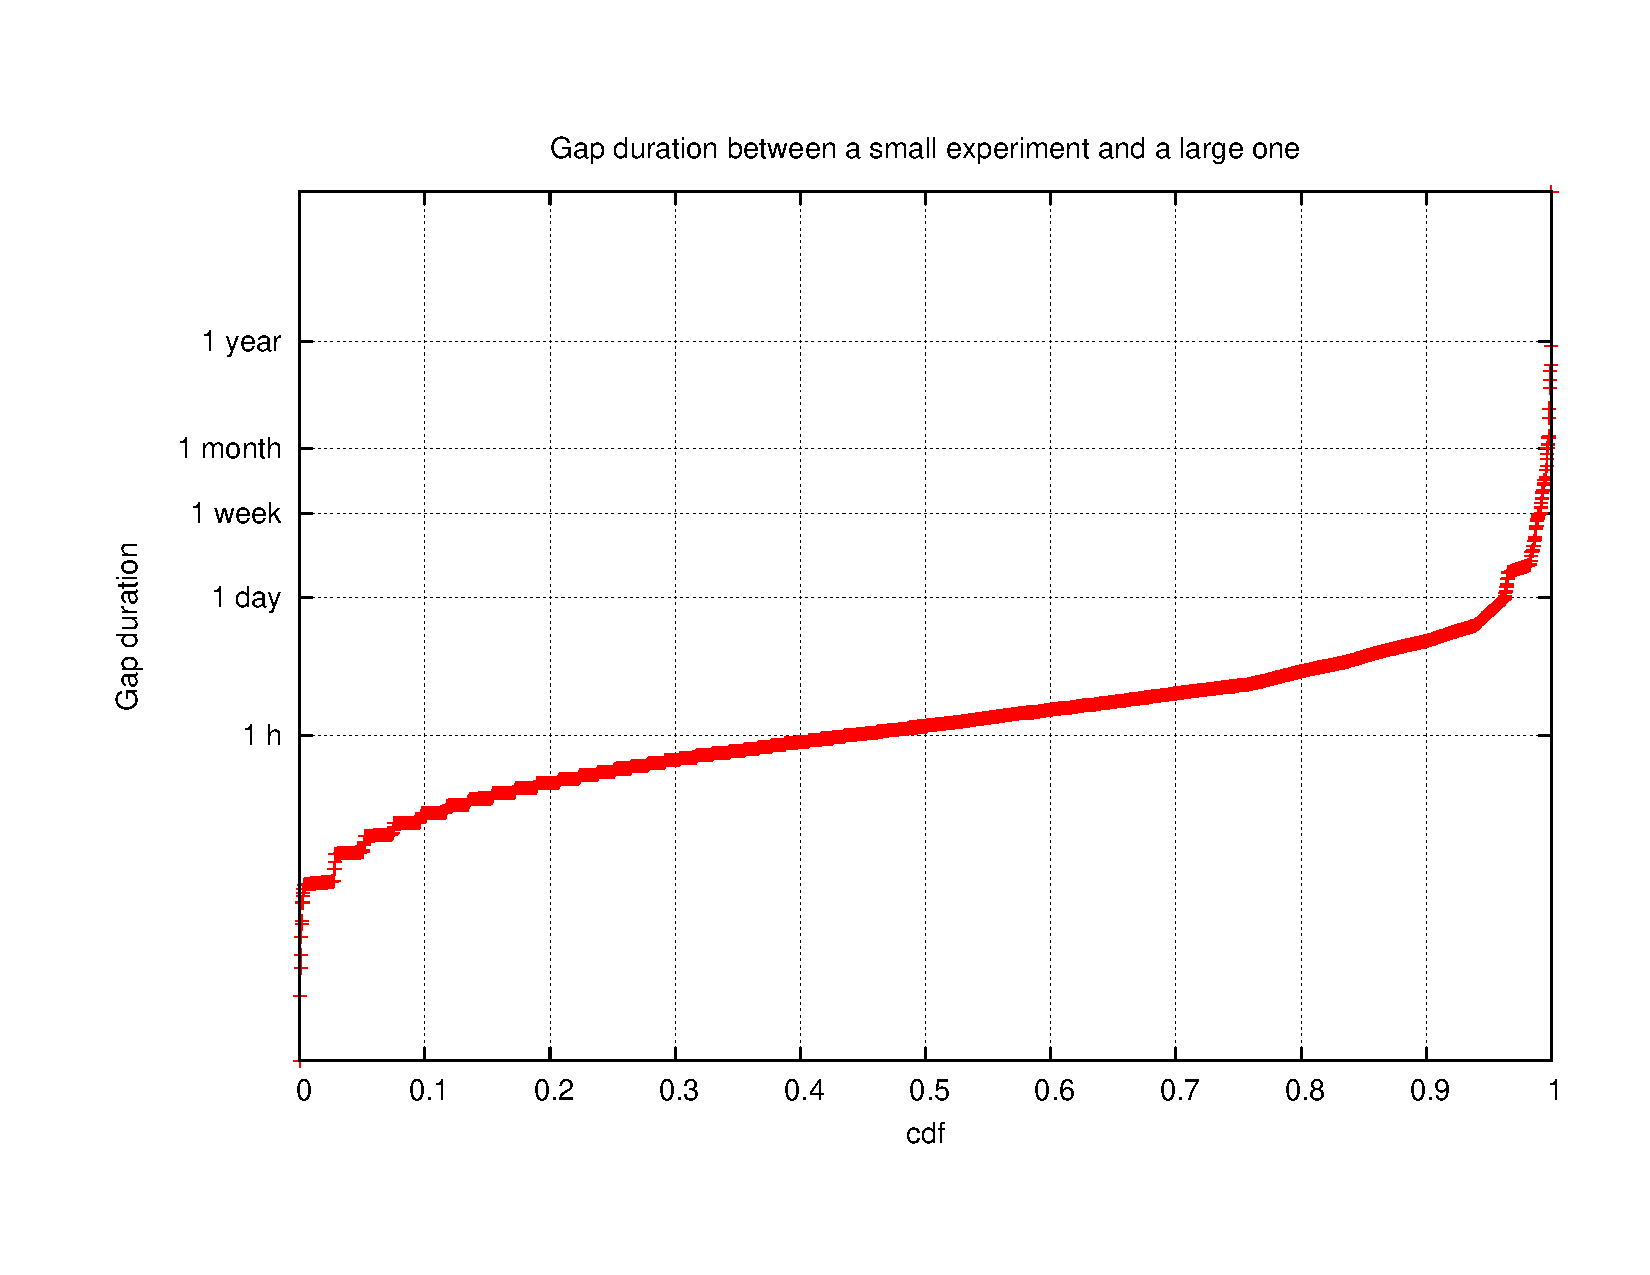
\includegraphics[width=5in]{figs/gaps.pdf}
\caption{Gap duration between a small experiment and a large one}
\label{gaps}
\end{center}
\end{figure}

\subsubsection{Project Size}
Figure~\ref{projsize} shows the project size in number of unique
experiments (one experiment can be allocated resources multiple times but it
still accounts for only one data point) for class and research projects.
We notice that most projects have a small number of experiments: 56\% of
research projects have less than 10 experiments and 23\% of class
projects have less than 10 experiments. Again this distribution is
heavy-tailed with a few projects generating hundreds of experiments.
Distributions of the number of allocations per project (Figure
\ref{projswap} exhibit are similarly heavy-tailed.

\begin{figure}[htbp]
\begin{center}
\includegraphics[width=5in]{figs/projsize.pdf}
\caption{Number of experiments per project}
\label{projsize}
\end{center}
\end{figure}

\begin{figure}[htbp]
\begin{center}
\includegraphics[width=5in]{figs/projswap.pdf}
\caption{Number of allocations per project}
\label{projswap}
\end{center}
\end{figure}

\subsubsection{Project Lifetime}
Figure \ref{projlife} shows the distribution of project lifetime,
from the first to the last event (experiment creation, resource allocation, resource release, modification). We notice that the smallest lifetime is 46 days,
with more than half of the research projects being active for more than
2.5 years and one third of class projects being active for more than a
year. Coupled with project activity data such as number of experiments
and number of resource allocation, and with experiment activity data such as
duration this shows that people use testbeds in multiple short visits
spread over a long time period.

Additionally, we found that
 a significant number of projects are created but never used,  that is, 
  not a single experiment is created within these projects. 
The percentages are: 24\% for DETER~\cite{Deter}, 24\% for Emulab~\cite{Emulab} 
 and 11\% for Schooner-WAIL testbeds~\cite{Wail}. 
We contacted the PIs of these unused DETER projects to understand their reasons for not using the 
 testbed and the responses we received can be broadly classified as: 
\begin{enumerate}
\item Found that simulation or live deployment are better fit with my research, 
\item Couldn't find sponsors or students for the project
\item Expected there was some specific software or hardware in the testbed, which proved wrong, and
\item Didn't really need to create experiments since the goal was simply to learn how to make a testbed on our own
\end{enumerate}
We are still investigating root causes of this phenomenon but the fact
that we observe these trends across very different testbeds points to the fact that
testbeds need better experimentation tools to eliminate many
cases under (1) and (3) categories. Having an ability to retire and resurrect projects would help 
better accounting by eliminating projects in (2) category and having a special project type for 
people that seek to build testbeds would eliminate projects in (4) category.

\begin{figure}[htbp]
\begin{center}
\includegraphics[width=5in]{figs/projlife.pdf}
\caption{Project lifetime}
\label{projlife}
\end{center}
\end{figure}

\subsection{User activity patterns}
User measures (TODO)


\subsection*{User Activity Patterns}
We define an "active" user as a user that has manipulated (created,
allocated, released, modified) an experiment within a project that
he belongs to. Figure \ref{projauser} plots the percentage of active users
in a project against the number of project members for research and
class projects. We notice that for small projects ($<$10 members for
research projects and $<$ 50 members for classes) percentage of active
users varies widely. The lowest percentage of active research users is
20\% while it is 3\% for class users. For large projects, however, a
large percentage of users is active. This effect is counterintuitive and
requires further investigation.

\begin{figure}[htbp]
\begin{center}
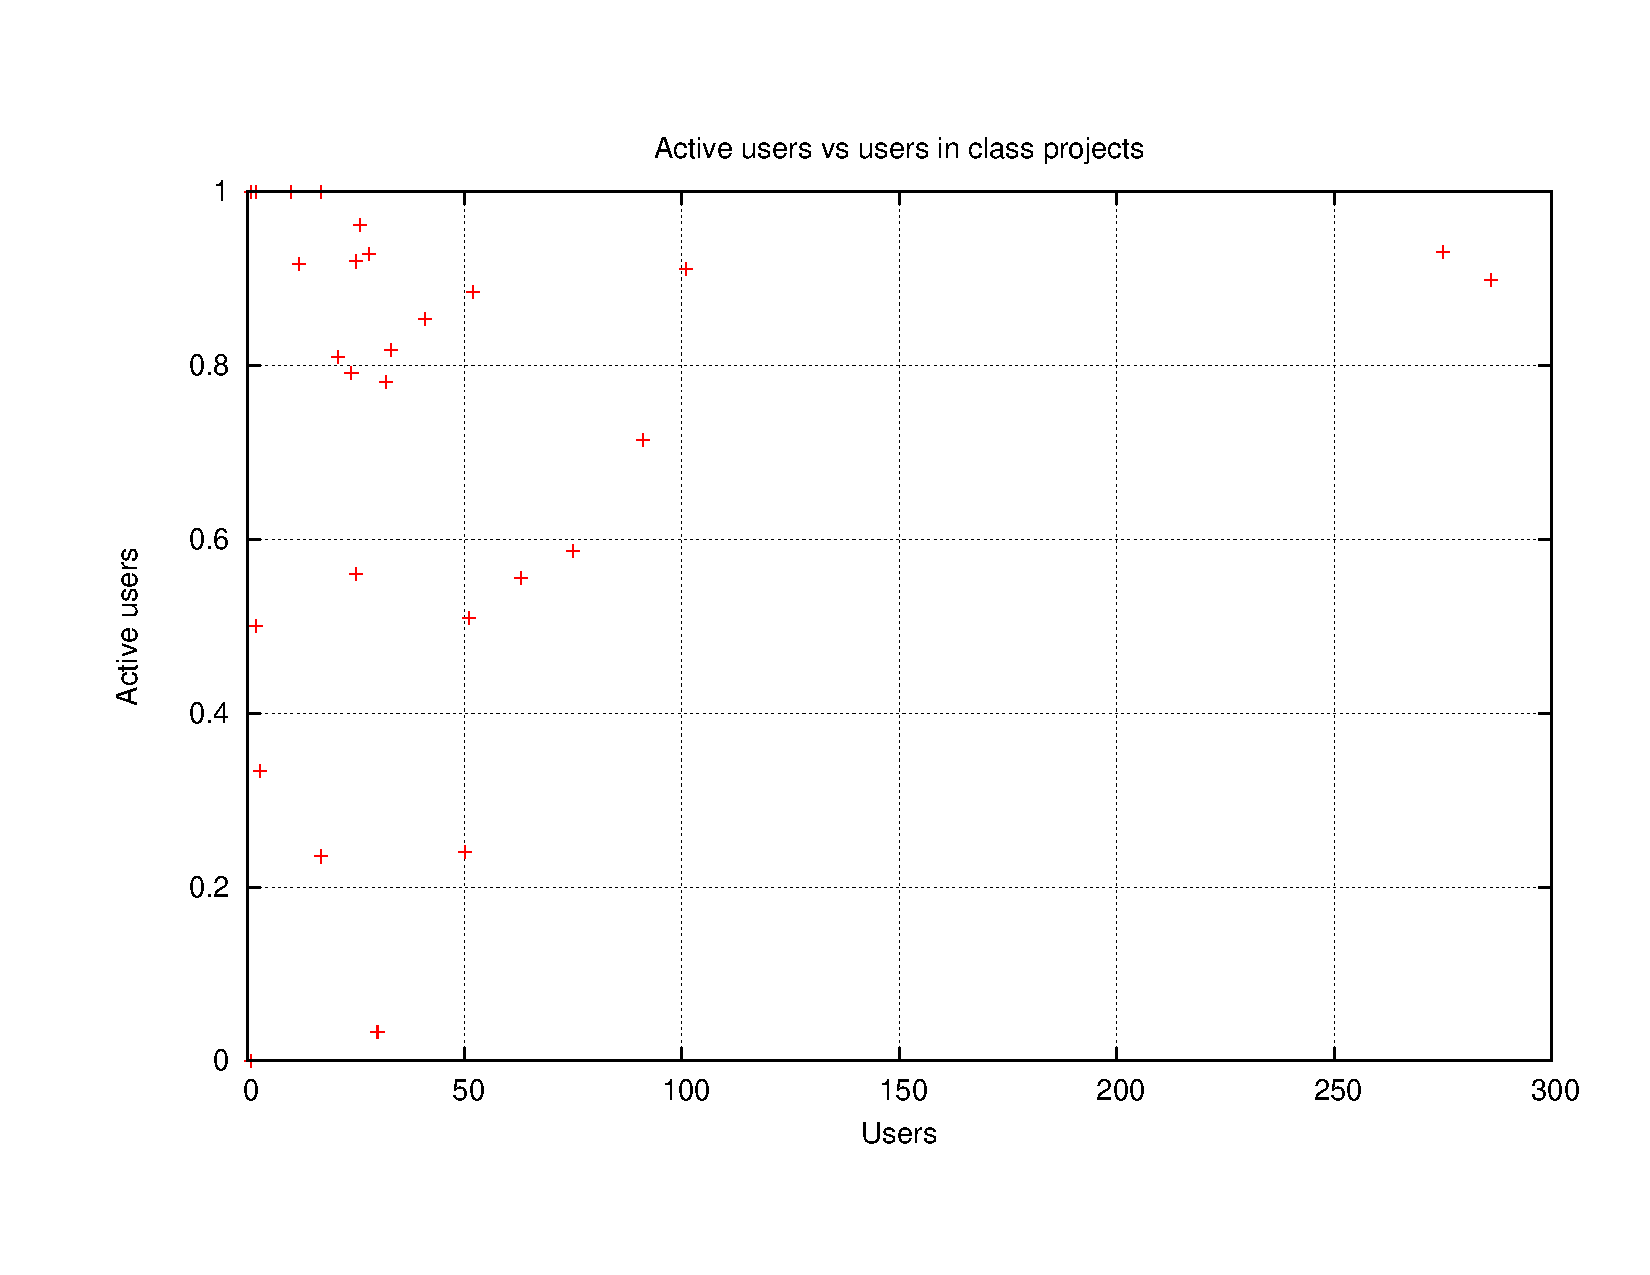
\includegraphics[width=5in]{figs/clprojauser.pdf}
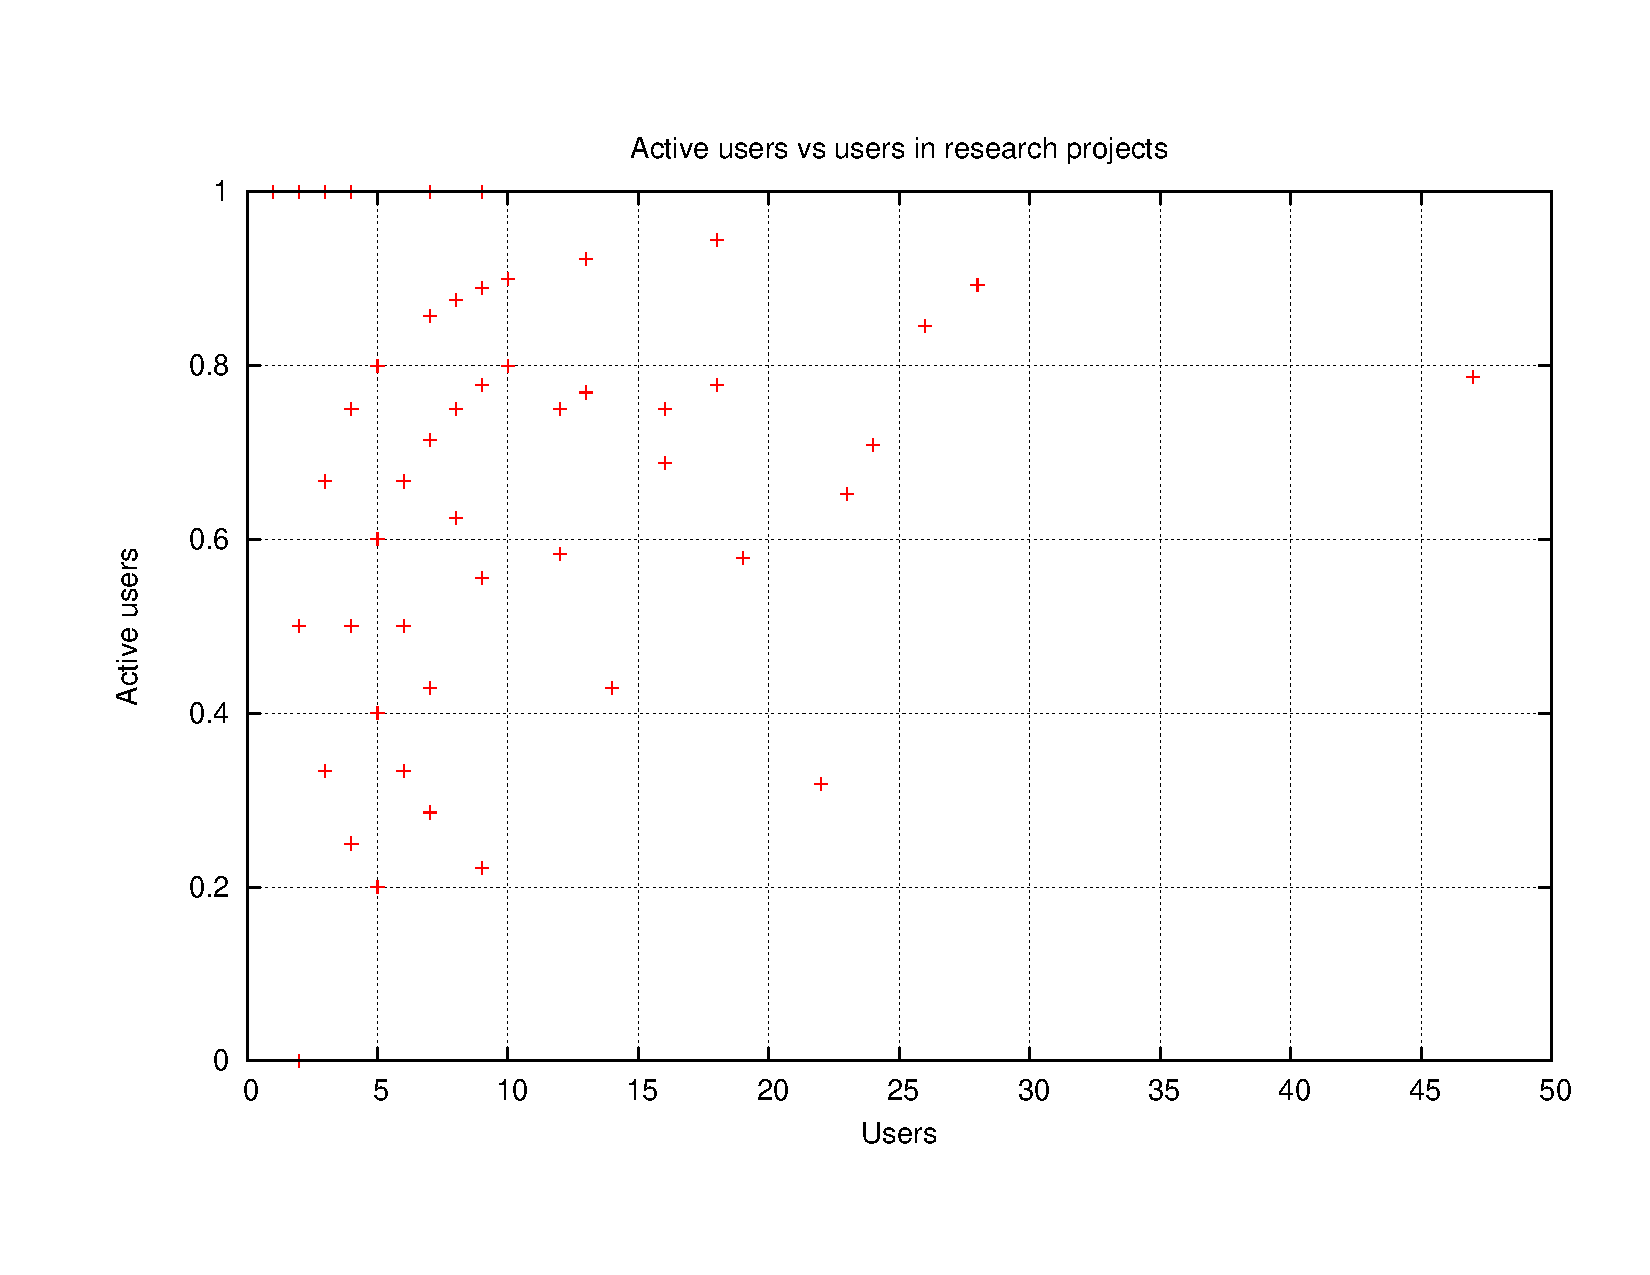
\includegraphics[width=5in]{figs/resprojauser.pdf}
\caption{Percentage of active users among all members in class and research projects}
\label{projauser}
\end{center}
\end{figure}

Additionally, we found 
 some number of users never manipulate 
  (create, allocate or release resources, modify) an experiment .
The percentages are: 10\% for DETER and 15\% for Schooner-WAIL. 
Closer investigation shows three causes of such behavior:
\begin{enumerate}
\item Users tend to open duplicate accounts if they forget their password and 
 can't retrieve it the regular way or if they change institution affiliation
\item PIs tend to create projects but do not manipulate experiments -- their students/employees do
\item Students in class projects may work with an experiment already 
 set up by the instructor or TA
\end{enumerate}
Cause (1) is preventable with better account management from testbed ops. Cause (2) can be easily identified and corresponding user records taken out of the statistics. Testbeds need better accounting to detect behavior due to cause (3). 

We now look deeper into these statistics. Figure \ref{uex} shows the number of unique experiments manipulated by a user. One unique experiment counts only once even if the user performed multiple runs of that experiment. Around half of research and class users manipulate less than five experiments. Around 90\% of research users manipulate 20 experiments or less, and 97\% manipulate 50 or less. Majority of class users (95\%) manipulate 10 experiments or less. 
 	
\begin{figure}[htbp]
\begin{center}
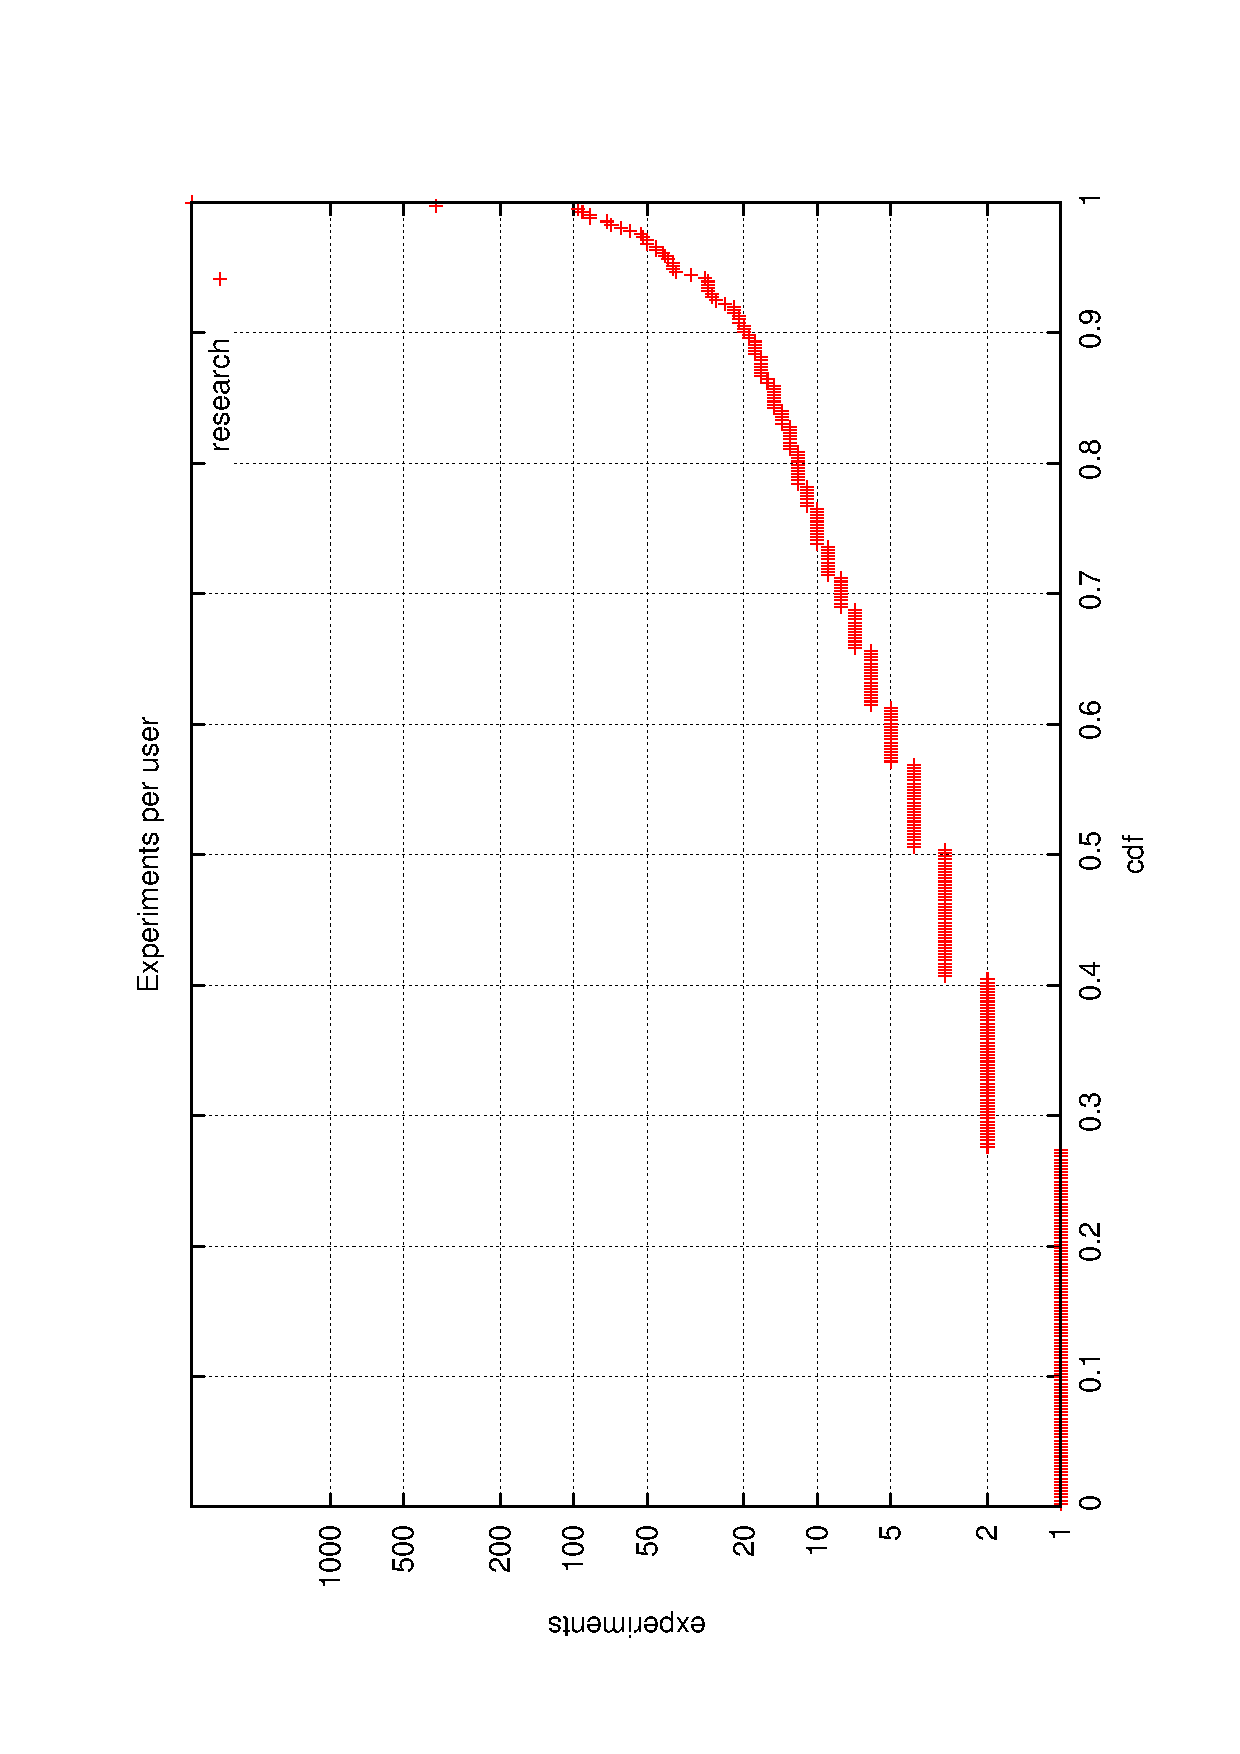
\includegraphics[width=5in]{figs/uex.pdf}
\caption{Experiments per user}
\label{uex}
\end{center}
\end{figure}

Figure \ref{uproj} shows the number of projects that a user belongs to. Around 90\% of research users and 97\% of class users belong to only one project. 
{\color{red} Check if multiple-project users are in fact PIs}

\begin{figure}[htbp]
\begin{center}
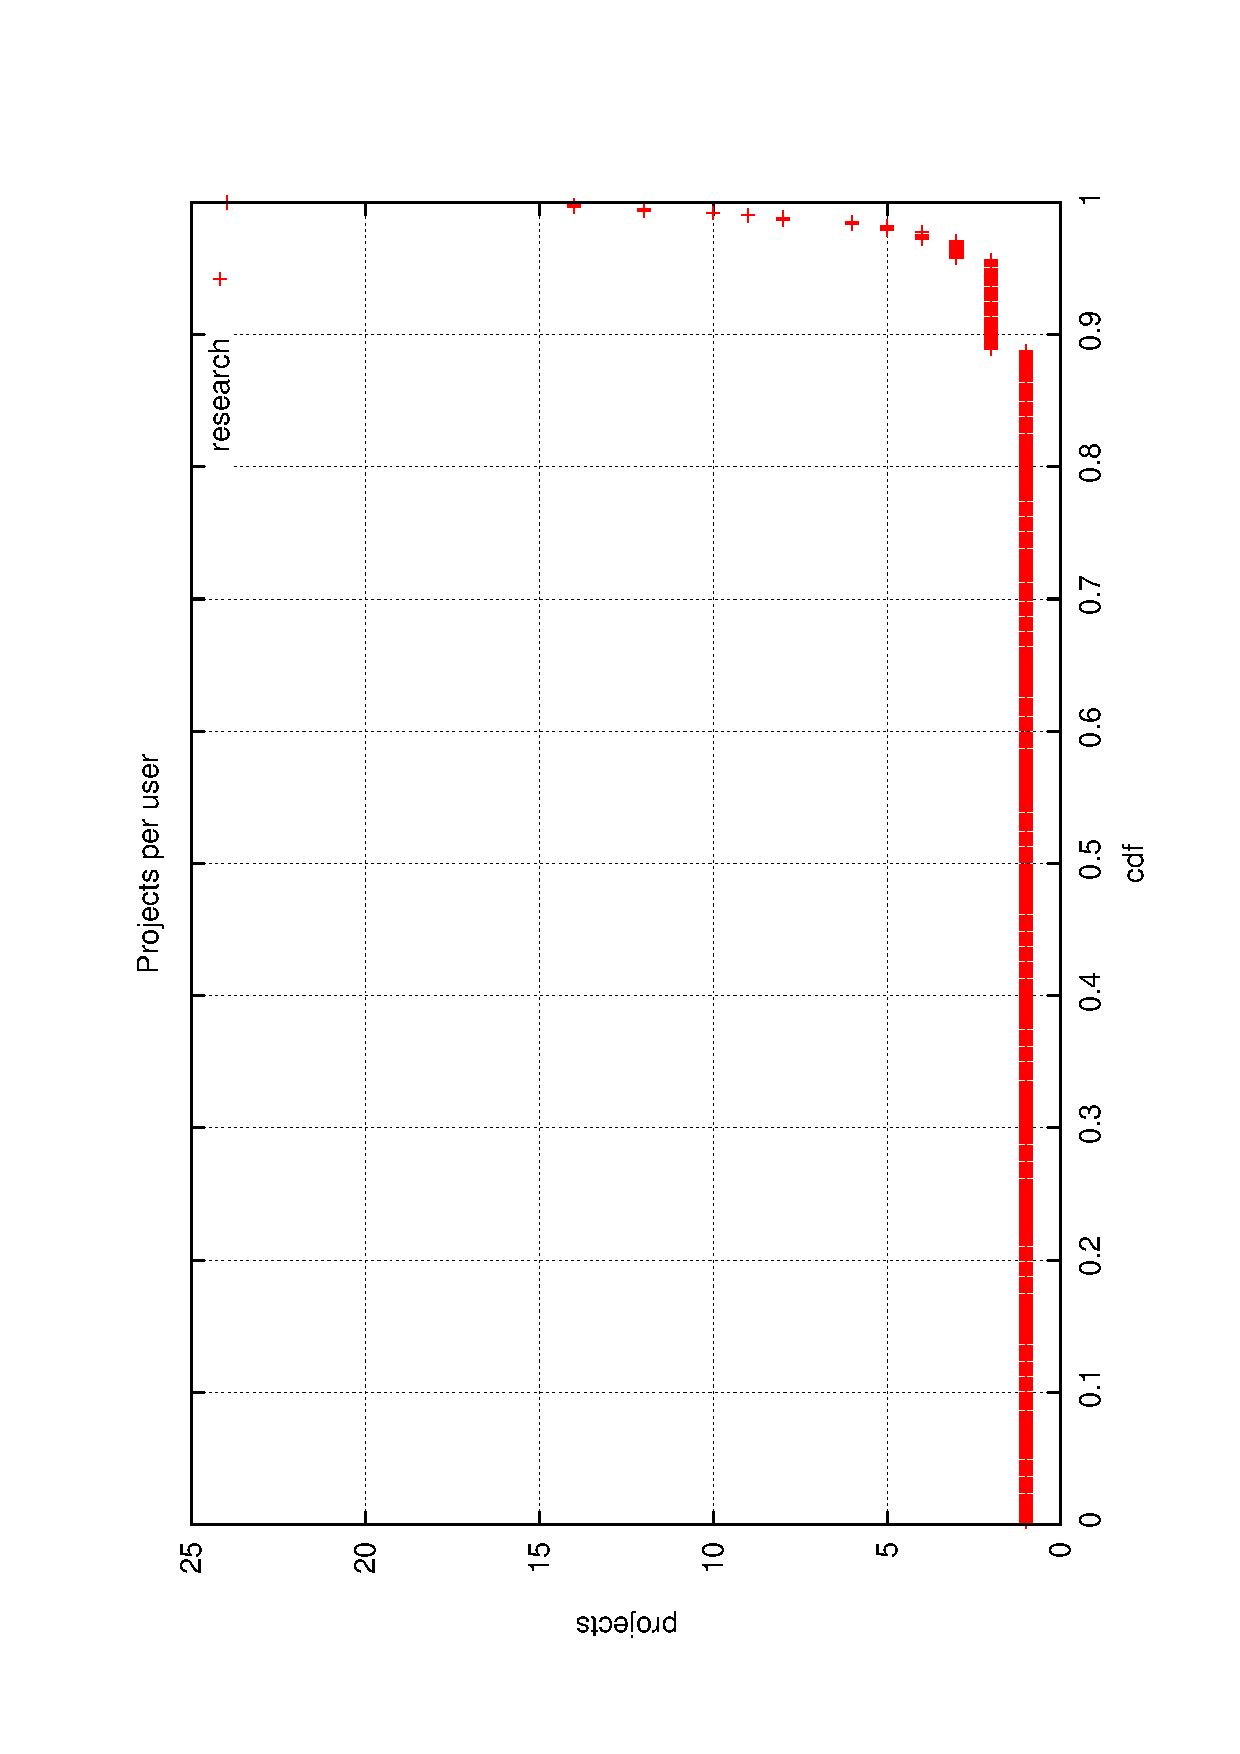
\includegraphics[width=5in]{figs/uproj.pdf}
\caption{Projects per user}
\label{uproj}
\end{center}
\end{figure}

Figure \ref{ulife} shows the distribution of a user's manipulation lifetime, i.e. it shows the elapsed time between the first and the last experiment manipulation by the user. Around 22\% of class users and 35\% of research users never manipulate an experiment, which is indicated by a lifetime on our x-axis. Half of research users and 35\% of class users are active for a week or less. Around 82\% of research users and almost all class users are active for a year or less. 
{\color{red} It's surprising that class users are longer active than research users -- investigate this further}

\begin{figure}[htbp]
\begin{center}
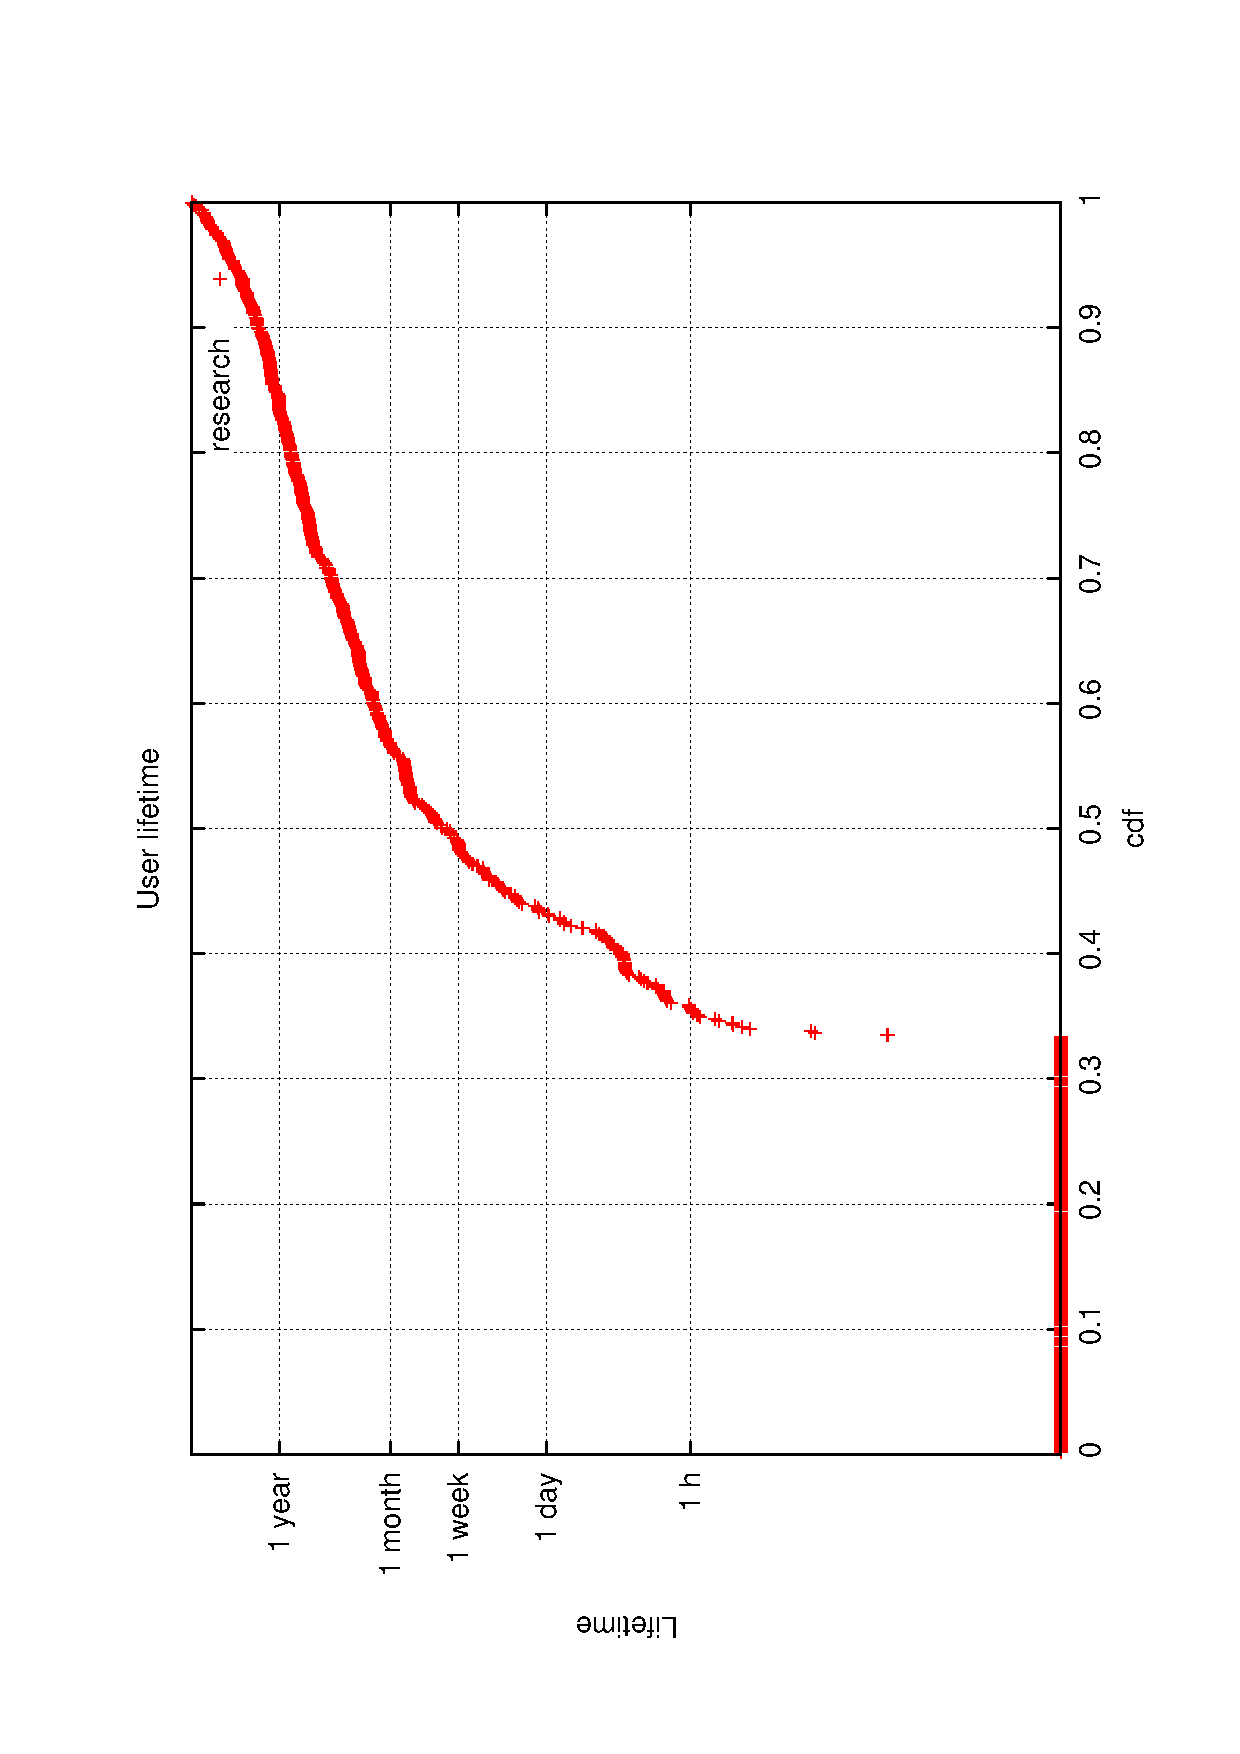
\includegraphics[width=5in]{figs/ulife.pdf}
\caption{User manipulation lifetime}
\label{ulife}
\end{center}
\end{figure}

We further define ``active lifetime'' of a user as the sum of all time when an experiment swapped in by this user was holding testbed resources. Figure \ref{uactive} shows the distribution of this time for research and class experiments. 60\% of class and research users are active for under one day. 90\% of class users are active for under two weeks, and 90\% of research users are active for under two months.

\begin{figure}[htbp]
\begin{center}
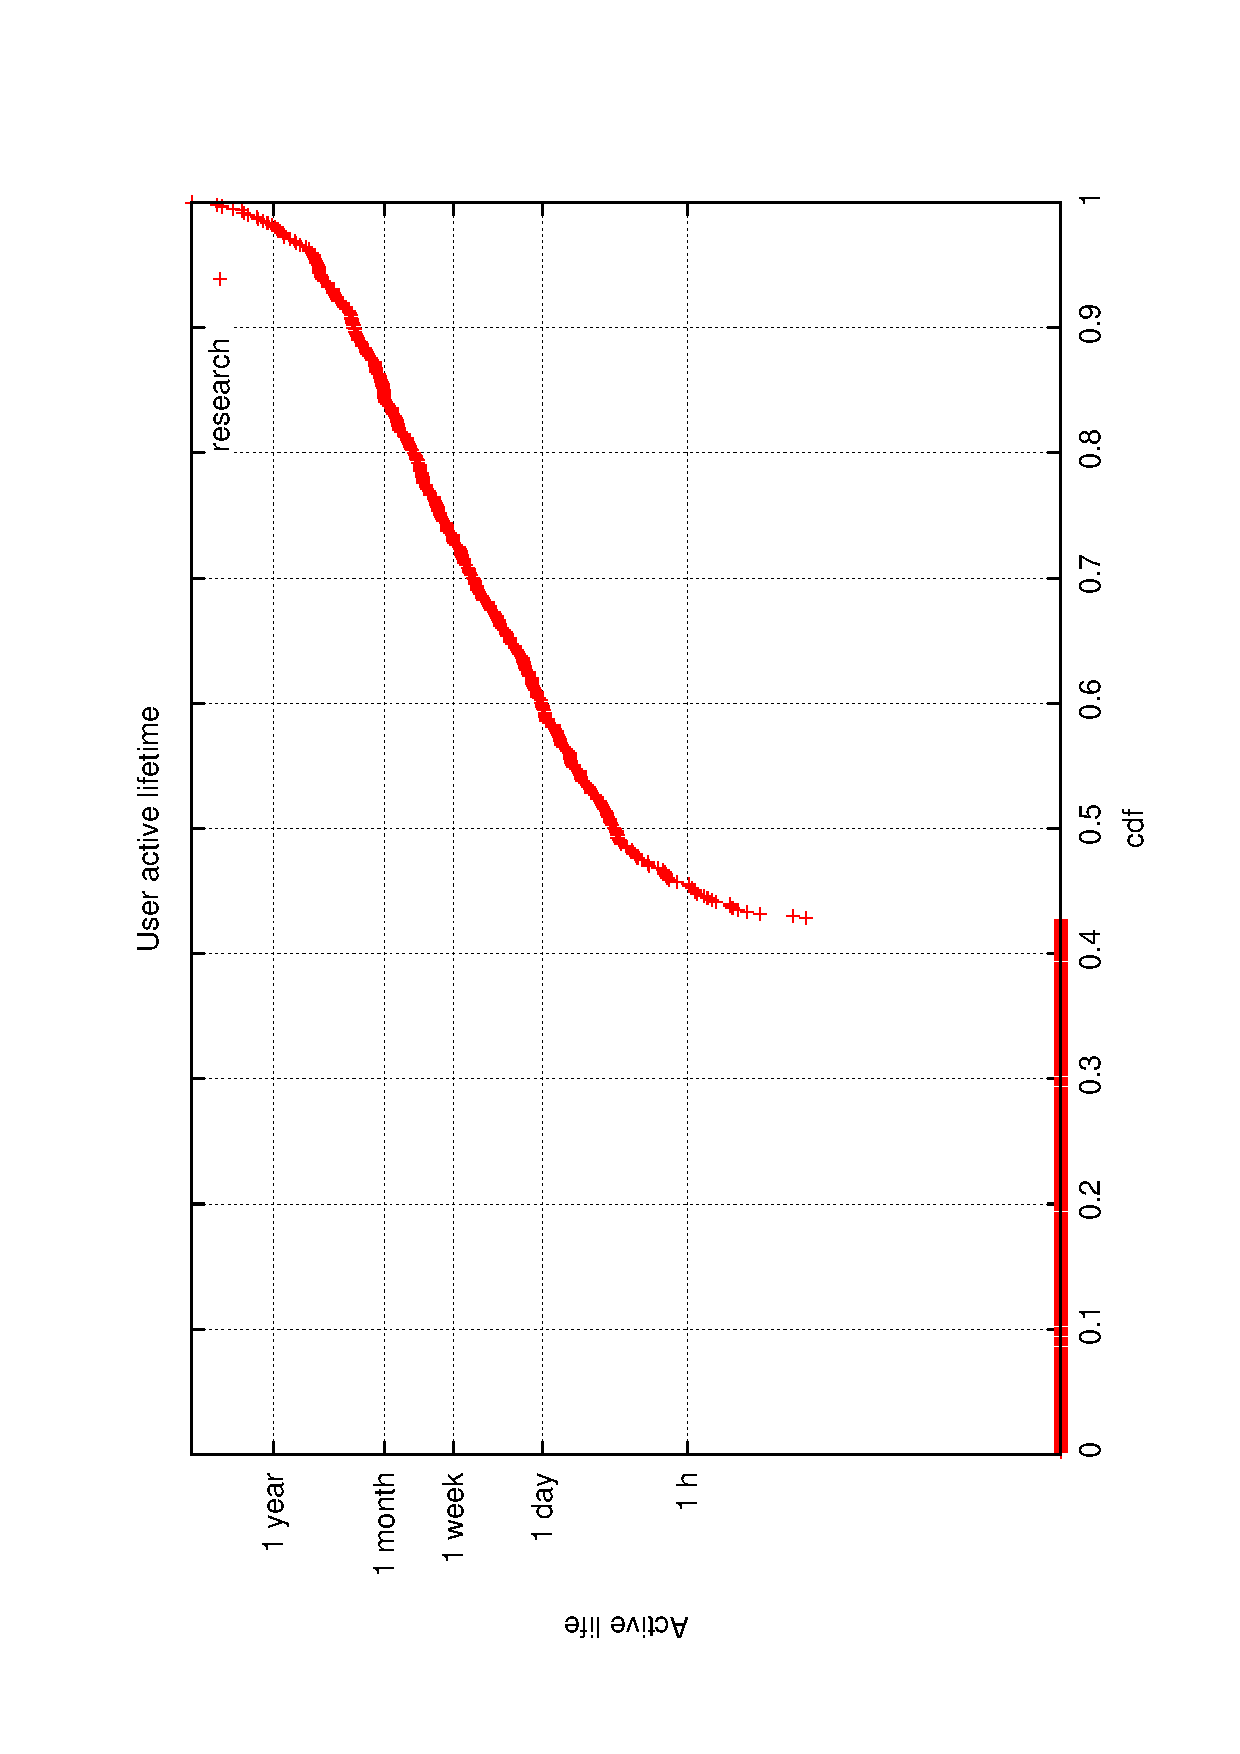
\includegraphics[width=5in]{figs/uactive.pdf}
\caption{User active lifetime}
\label{uactive}
\end{center}
\end{figure}

\subsection{Idleness}
{\color{red} Explain that we want to investigate how well are resources used and if we could have a better idle-swap policy to serve more users. }
{\color{red} Explain how we calculate idle time and how we gather statistics. }

These are statistics from September 13, 2010 to April 1, 2011. 
54\% of timeslots had a free node that was not allocated to an experiment. 
26\% of timeslots had an idle node. 12\% had a node with only a network activity,
3\% had a node with only a CPU activity and 1\% had a node with network and CPU activity.

We next seek to understand the cause for idleness and look for two different patterns: (1) instances where some nodes 
in an experiment were never used and (2) instances where all nodes in an experiment were idle for some time. We now treat
class and research projects together.

Only 0.5\% of experiment instances had one or more idle nodes. This means that users can usually estimate well 
what size of network they need for experimentation. 

\begin{figure}[htbp]
\begin{center}
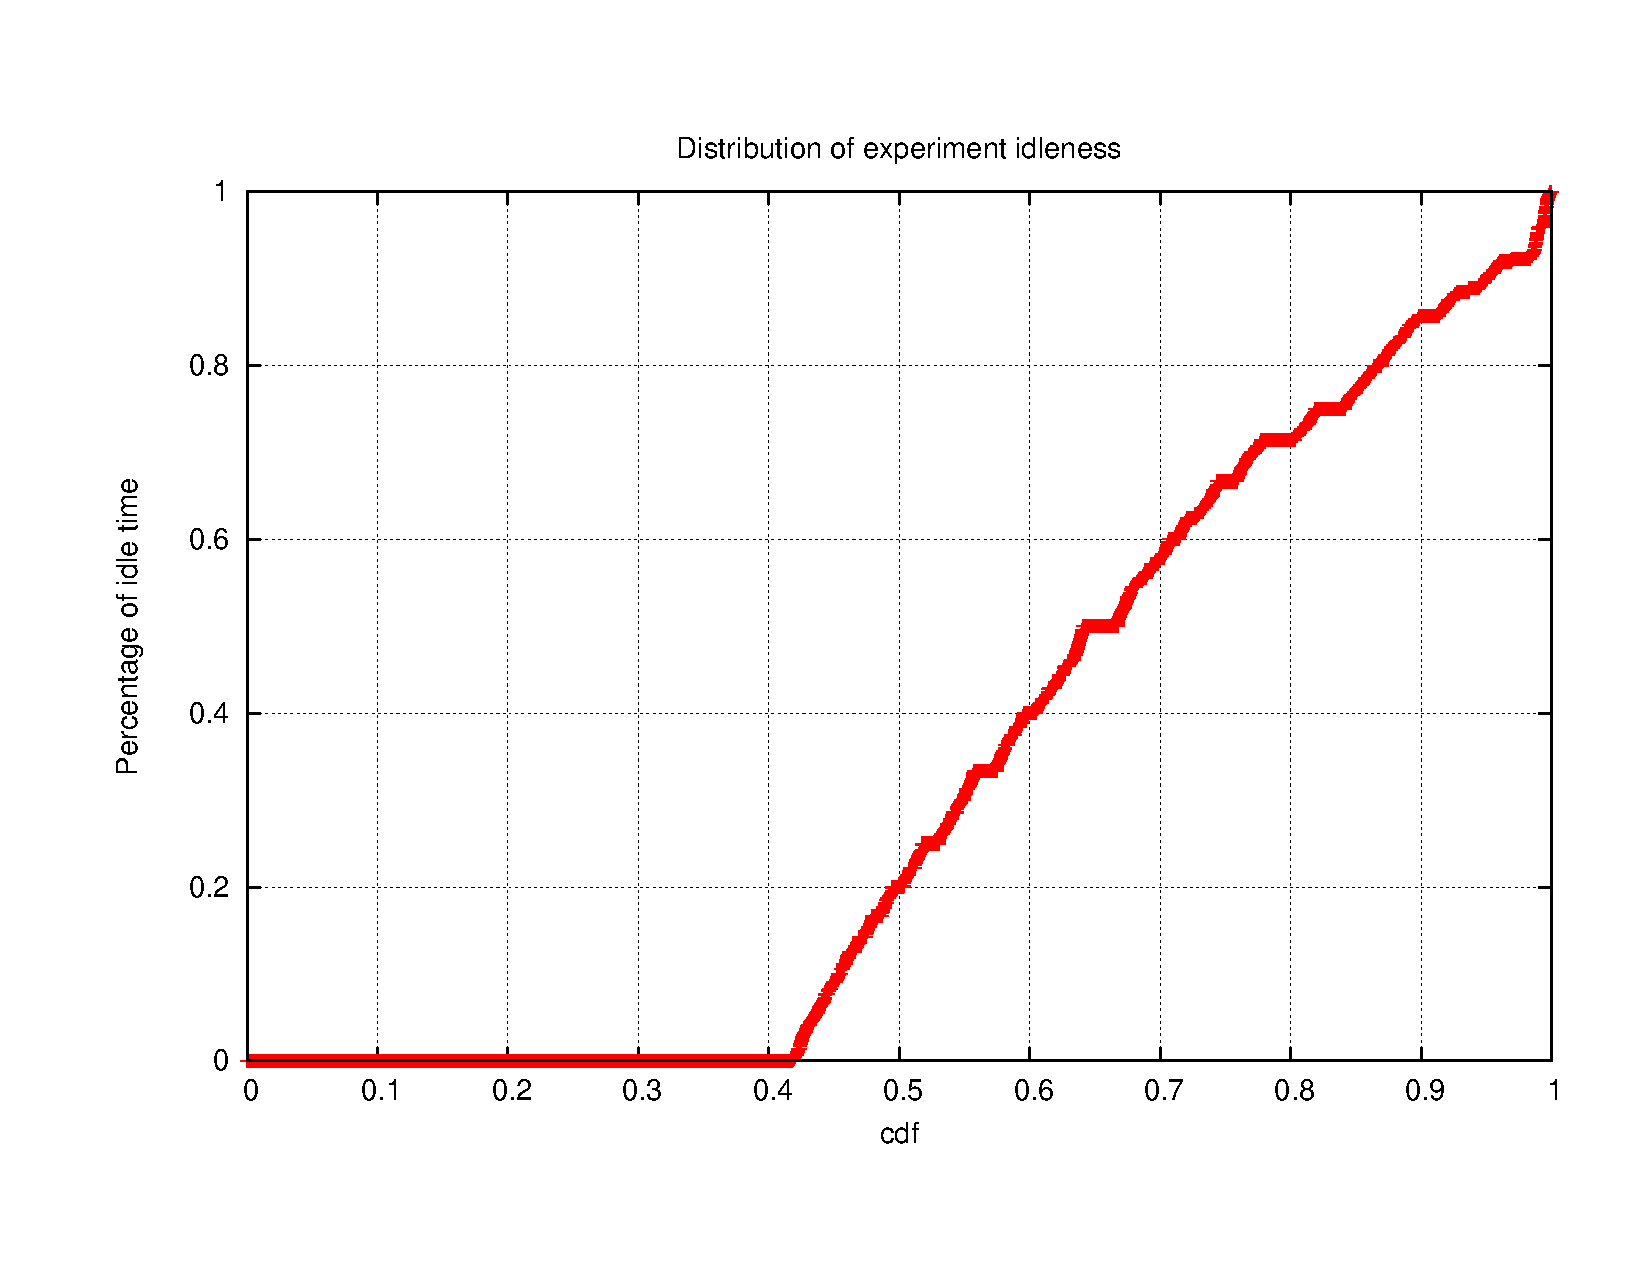
\includegraphics[width=5in]{figs/timeidle.pdf}
\caption{Distribution of experiment idleness}
\label{timeidle}
\end{center}
\end{figure}

Figure \ref{timeidle} shows the distribution of the percentage of idle time in an experiment. A little more than 40\% of experiments are never idle. The idleness distribution then changes almost linearly until it reaches 100\%. 

\begin{figure}[htbp]
\begin{center}
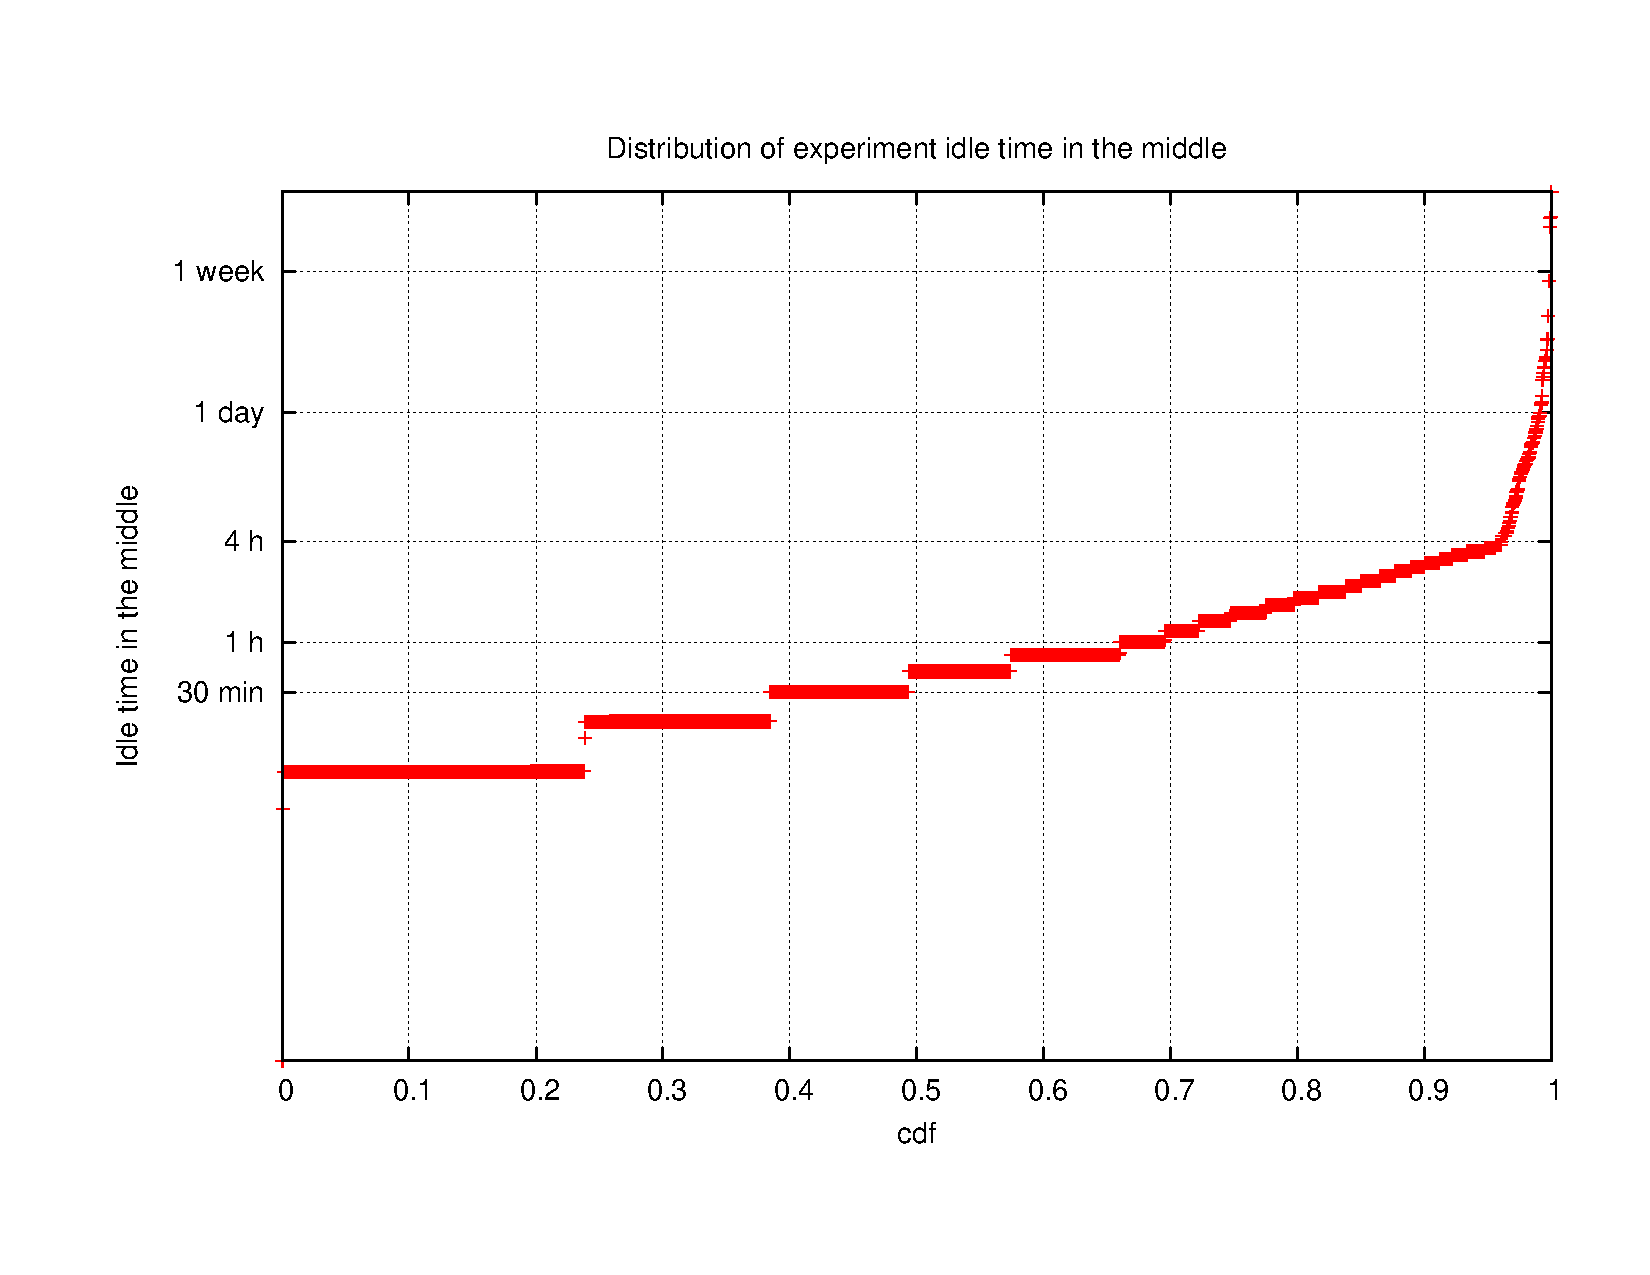
\includegraphics[width=5in]{figs/mididle.pdf}
\caption{Distribution of experiment idle time in the middle}
\label{mididle}
\end{center}
\end{figure}

We further investigate the duration of idle gaps seeking to understand if testbeds could be better utilized if idle experiments were auto-swapped out after only a brief idle time and swapped back in later. 
Figure \ref{mididle} shows the longest idle interval for each experiment, where the number of idle timeslots was positive. Around 65\% of experiments are idle less than 1h, and 96\% of them are idle less than 4h. This means that the idle-swap time set at 4h is a good estimate. 

\begin{figure}[htbp]
\begin{center}
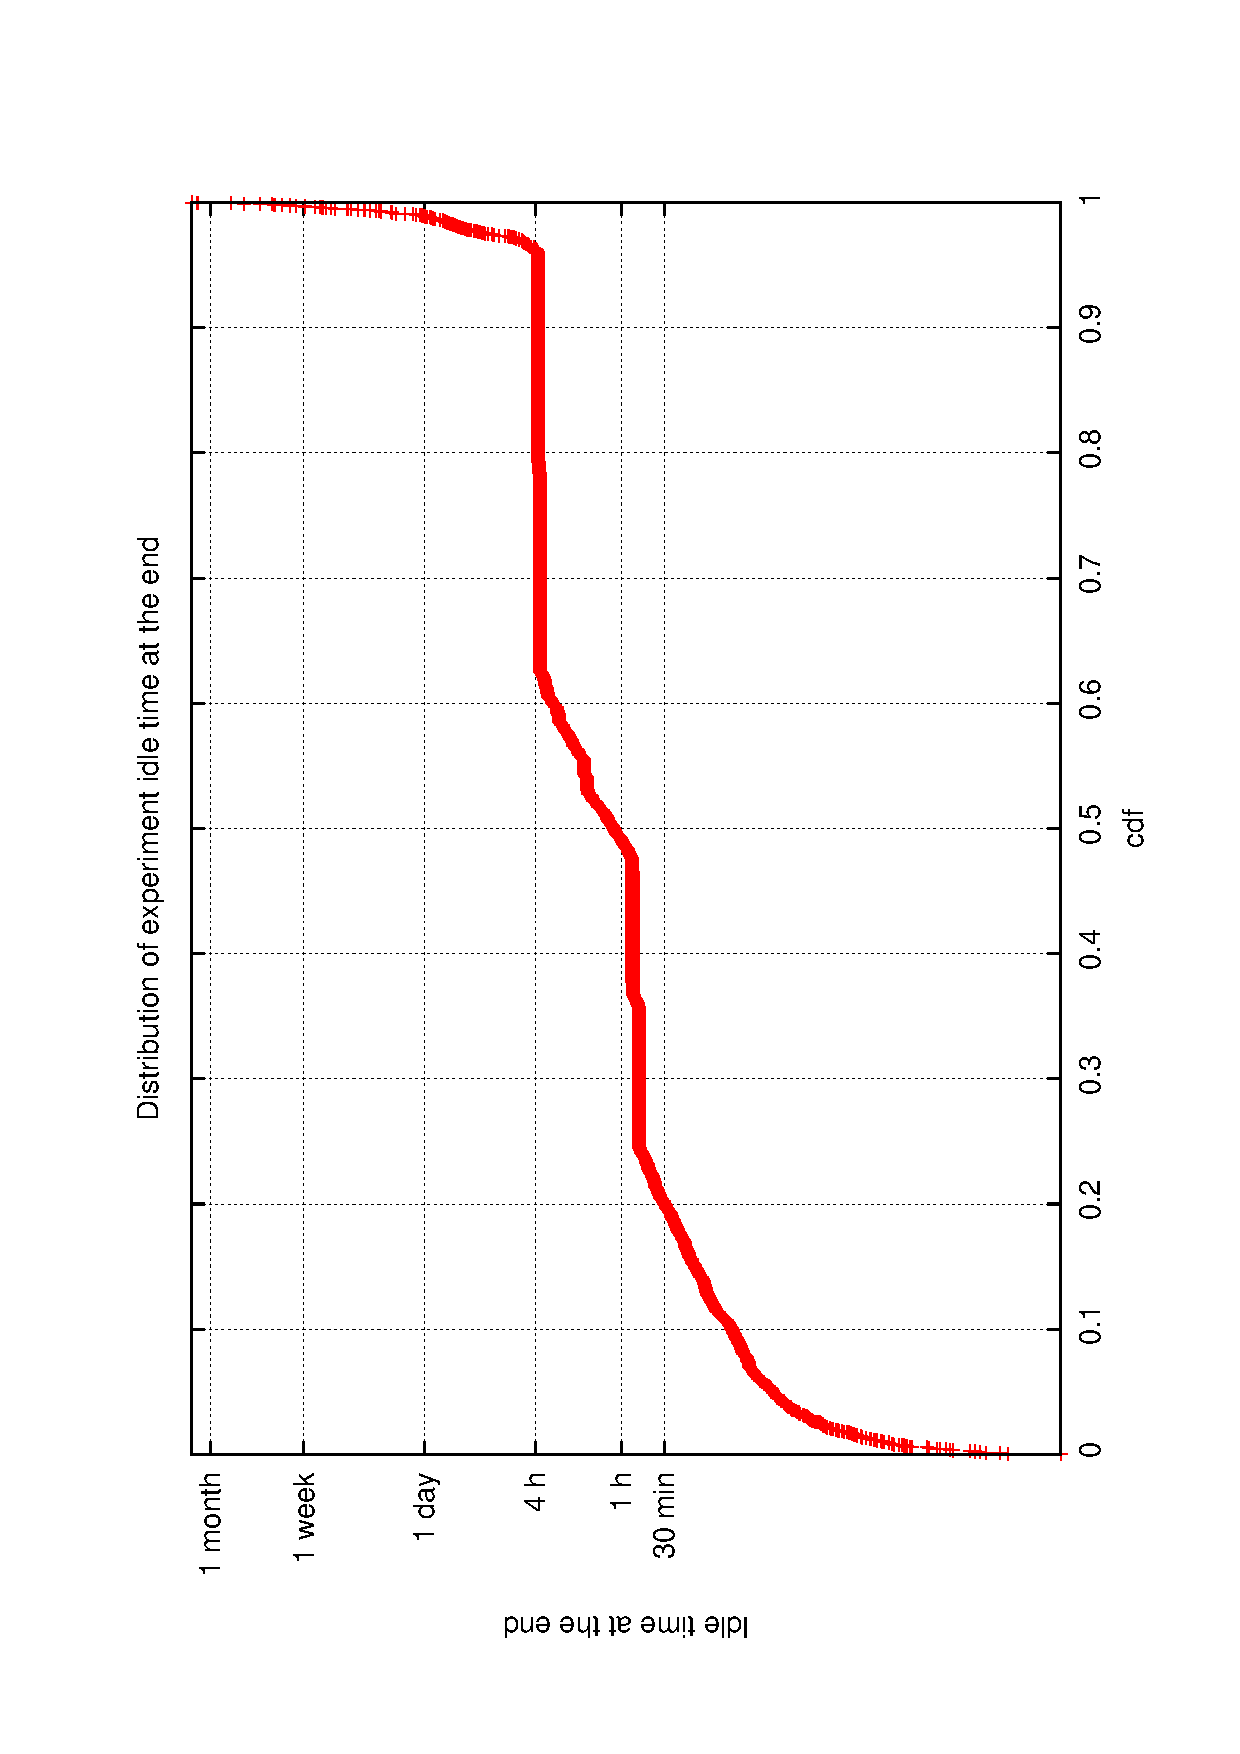
\includegraphics[width=5in]{figs/endidle.pdf}
\caption{Distribution of experiment idle time at the end}
\label{endidle}
\end{center}
\end{figure}

Figure \ref{endidle} shows the duration of the idle interval before the experiment is swapped out. About a quarter of experiments are idle less than 1h before being swapped out. There is an almost flat line near the 1h mark going from 25\% to near 50\% of experiments. These are mostly class experiments for which the idle-swap time is automatically set to 1h. A similar flat line is visible around 4h from 62\% to 96\%. These are research experiments for which the idle-swap time is automatically set to 4h. Again these figures mean that our settings are correct. 


{\color{red} Failed swapin data (TODO)}

{\color{red} Planetlab (TODO)}

{\color{red} Starbed (TODO)}

\section{Experiment Characteristics}

Topology (TODO)

OS (TODO)

Link characteristics (TODO)

SEER (TODO)

\section{What hinders testbed use}
 
Survey results (TODO)

\section{Implications for the Future}

\section{Conclusions}

\end{document}
